%----------------------------------------------------------------------------------------
%	PACKAGES AND OTHER DOCUMENT CONFIGURATIONS
%----------------------------------------------------------------------------------------

\documentclass[12pt]{article}
\usepackage[english]{babel}
\usepackage[utf8x]{inputenc}
\usepackage{amsmath}
\usepackage{graphicx}
\usepackage[colorinlistoftodos]{todonotes}
\usepackage{ragged2e}
\usepackage[none]{hyphenat}
\usepackage[hidelinks]{hyperref}
\usepackage{listings}
\usepackage[title,titletoc,toc]{appendix}
\usepackage{kantlipsum}
\usepackage{spverbatim}
\usepackage{caption3}
\usepackage{longtable}
\usepackage{alltt}
% This is for adding extra subsections
\usepackage{titlesec}
\titleclass{\subsubsubsection}{straight}[\subsection]
\newcounter{subsubsubsection}[subsubsection]
\renewcommand\thesubsubsubsection{\thesubsubsection.\arabic{subsubsubsection}}
\renewcommand\theparagraph{\thesubsubsubsection.\arabic{paragraph}}
\renewcommand\thesubparagraph{\theparagraph.\arabic{subparagraph}}

\usepackage{chngcntr}
\counterwithin{figure}{section}

\titleformat{\subsubsubsection}
  {\normalfont\normalsize\bfseries}{\thesubsubsubsection}{1em}{}
\titlespacing*{\subsubsubsection}
{0pt}{3.25ex plus 1ex minus .2ex}{1.5ex plus .2ex}

\makeatletter
\renewcommand\paragraph{\@startsection{paragraph}{5}{\z@}%
  {3.25ex \@plus1ex \@minus.2ex}%
  {-1em}%
  {\normalfont\normalsize\bfseries}}
\renewcommand\subparagraph{\@startsection{subparagraph}{6}{\parindent}
  {3.25ex \@plus1ex \@minus .2ex}%
  {-1em}%
  {\normalfont\normalsize\bfseries}}
\def\toclevel@subsubsubsection{4}
\def\toclevel@paragraph{5}
\def\toclevel@paragraph{6}
\def\l@subsubsubsection{\@dottedtocline{4}{7em}{4em}}
\def\l@paragraph{\@dottedtocline{5}{10em}{5em}}
\def\l@subparagraph{\@dottedtocline{6}{14em}{6em}}
\@addtoreset{subsubsubsection}{section}
\@addtoreset{subsubsubsection}{subsection}
\@addtoreset{paragraph}{subsubsubsection}
\makeatother
\setcounter{secnumdepth}{4}
\setcounter{tocdepth}{5}


%-----------------------------------------------%

%Add package for acronyms

% Load the package
\usepackage{glossaries}
 
% Generate the glossary
\makeglossaries
%-------------------------------------------------

\usepackage{array}
\newcolumntype{L}[1]{>{\raggedright\let\newline\\\arraybackslash\hspace{0pt}}m{#1}}
\newcolumntype{C}[1]{>{\centering\let\newline\\\arraybackslash\hspace{0pt}}m{#1}}
\newcolumntype{R}[1]{>{\raggedleft\let\newline\\\arraybackslash\hspace{0pt}}m{#1}}

\begin{document}

\begin{titlepage}

\newcommand{\HRule}{\rule{\linewidth}{0.5mm}} 
\center

%----------------------------------------------------------------------------------------
%	LOGO SECTION
%----------------------------------------------------------------------------------------


\includegraphics{images/uva.jpeg}\\[0.5cm]% Include a department/university logo - this will require the graphicx package
 
%----------------------------------------------------------------------------------------

%----------------------------------------------------------------------------------------
%	HEADING SECTIONS
%----------------------------------------------------------------------------------------
\textsc{\Large System and Network Engineering, MSc}\\[0.5cm] 
\textsc { \large Research Project 1}\\[0.4cm] % Title of your document

%----------------------------------------------------------------------------------------
%	TITLE SECTION
%----------------------------------------------------------------------------------------
\HRule \\[0.4cm]
{ \huge \bfseries Security Intelligence Data Mining}\\[0.4cm] % Title of your document
{ \large \bfseries Research Proposal}\\[0.4cm] % Title of your document
\HRule \\[0.4cm]




%----------------------------------------------------------------------------------------
%	AUTHOR SECTION
%----------------------------------------------------------------------------------------


\large Diana Rusu\\
{\bfseries Diana.Rusu@os3.nl}\\[0.5cm]
\large Nikolaos Petros Triantafyllidis\\
\bfseries Nikolaos.Triantafyllidis@os3.nl\\[2cm]

{\large \today} 

\end{titlepage}

\newpage
\begin{abstract}
\noindent
This project deals with gathering Intelligence about IT Security incidents by mining data originating from the public Web. Our aim is to propose the architecture of a software system that is able to collect, preprocess and mine public information as well as alert and assess the threat level. \\
\\
A small Proof of Concept implementation for the proposed System Architecture is an outcome of this research. 
\end{abstract}
\newpage
\section*{Acknowledgements}

We would like to express our gratitude and appreciation towards certain people that helped us during this Research Project as well as our studies so far, for all the support, expert knowledge and guidelines they provided. 
\hfill \break \\ 
First of all we would like to thank Delloite Netherlands, for granting us access to their headquarters building, and providing us with all the resources needed for the completion of our research. We owe utmost gratitude to all the employes of Deloitte NL that took time out of their busy schedule to assist us with our project. 
\\ 
To begin with we would like to thank mr.Henri Hambartsumyan who came up with the idea of this project and who was the our first contact with the company. \\
To our main supervisor mr.Joost Kremers we express our warm thanks for always being there to assist us and provide feedback, even if his schedule would not permit it. Even before we started working on this project he made sure to guide and direct us to the right research path.\\
Next we feel the need to thank the developers of the CTI portal, mr.Niels Pompe for providing us with a list of Web resources relevant to our project and introducing us to the rest of the CTI team. Mr.Ari Davies, for guiding our development effort and mr. Gijs Hollestelle for explainingt the usage of their platform and explained to us the further needed requirements.\\
Last but not least we would like Vincent van de Ven from the Data Analytics team, for providing us valuable insights about Data Management techniques. 
\hfill \break \\ 
Secondly, we would like to thank the University of Amsterdam and the people from the OS3 core team for their support during our studies. Dr.Cees de Laat, co-ordinator of the Research Projects, our professors dr.Karst Koymans and dr.Jaap van Ginkel as well as our lab teachers dr. Arno Bakker and dr.Jeroen van der Ham. 
\hfill \break \\ 
This has been a great opportunity for us to experience working with a large multinational company in a real business environment, even for this short period of time.

\newpage

\tableofcontents
\newpage

\section{Introduction (NEEDS REVISION)}
%\addcontentsline{toc}{section}{Introduction}
\parbox{\linewidth}{
With the increasing number of cyber-attacks and the growth of computer crime worldwide, it becomes apparent that IT security is a major concern and crucial survival factor for large companies, organisations and institutions of any sort. Security Operations departments working to ensure confidentiality, integrity and availability for the system infrastructure of their organisation, invest huge  parts \cite{cyber} of their time and effort in detecting threats in real time. A very valuable source of security intelligence, vital to cyber-risk assessment, is information mined from data posted on public sites such as "pastebins" or social networks. However, this is a very cumbersome task due to the lack of Natural Language Processing capabilities in most of the existing tools.\hfill \break \\
The aim of our research is to propose a system that is capable of detecting possible security threats and creating alerts about incidents by applying Data Mining tasks on data collected from various different public Web sources, that have been further structured and filtered. The system must be configurable in order to include \hfill \break \\
For each distinct part in the proposed System Architecture, we define its specifications and give 

This project was proposed by and carried out in co-operation with Deloitte Netherlands. 
}
\newpage
\subsection{Research Questions}
This topic is admittedly very open but it can be narrowed down to several specific research questions some of which we will try to answer to some extent. The main question that we will be trying to answer is the following:\\[0.1cm]

\noindent
\textbf{How can we effectively use public sources to obtain real time information about security incidents?}\\[0.1cm]

\noindent
This question can be analysed into more specific parts that cover the topic to some extent, as follows:

\begin{enumerate}
	\item How can the raw data be effectively collected from the public sources? 
	\begin{itemize}
		\item How can we effectively detect the reliable sources?
		\item What search terms can we deploy during the retrieval phase?
		\item How can the unstructured data be pre-processed? 
	\end{itemize}
	\item How can the data be analysed in respect to security operations?
	\begin{itemize}
		\item How can we apply current Data Mining and Analytics techniques on Security issues?
		\item How can we derive the risk assessment model from the above?
		\item How can we apply the model on new data?
	\end{itemize}
	\item	How can the collected knowledge be applied on a system implementation?
	\begin{itemize}
		\item What is a reliable and extensible System Architecture that can be designed?
		\item What are the computational and storage requirements of such a system?
		\item What extensions can be proposed for that system?
	\end{itemize}
\end{enumerate}

The proposed system extensions can spawn further research questions, namely on the topics of presenting the analysed data, reacting to the real time events and finally assessing the situations that arise and providing feedback to the system.


\subsection{Related work}
There is a lot of literature around the field of Data Mining and more recently Web Mining. The most prominent and recent case is the book 'Mining The Social Web' by M.Russel \cite{socialweb} that deals with exploring and mining information from social websites (e.g., Facebook, Twitter, LinkedIn, Google+, GitHub, etc.). There are also several academic papers and books that deal with applying Data Mining to System Security. One example is a system proposed by the university of Minnesota, called MINDS, that employs various Data Mining in Intrusion Detection. The system is described in their paper 'Data Mining for Cyber Security' \cite{minds}.  Another example is a system proposed by the Dutch company Sentient in co-operation with the Amsterdam Police Force \cite{police} aiming to provide Data Analytics operations automation while on the same time minimising the technical expertise needed by the system user. 
\subsection{Ethical implications}

The main part of this research comprises of exploring current techniques and their application on IT security, as well as the specification of a system that employs Data Mining techniques to collect security intelligence. In order for the models to be defined some amount of information will have to be gathered. This information will originate solely from public sources and will be mostly historical data. In the unlikely case that any previously unnoticed security issues are encountered they will be handled with discretion and communicated only towards the appropriate targets and only with the approval of the OS3 core team and Deloitte Digital. The collection or storage of personal data is not intended and any collected information will be discarded after the end of this project. The usage of shared computational and network infrastructure will only be used for the needs of this project and within the legal limits.

\newpage
\section{Methodology and Results}
This project was carried out in collaboration with Deloitte Risk Services, Netherlands. We first got acquainted with the Cyber-Risk Services team and were introduced to the effort already carried out towards the development of a Cyber Threat Intelligence (CTI) system. \\
Based on the expert knowledge collected we defined the parts needed for complementing the portal developed by Deloitte, in order to derive a generalised System Architecture. The next step was to start developing the building blocks of the System to a level that would allow the creation of a functional Proof of Concept. We first developed Data Aggregators for four distinct data sources. We then looked into methods for determining the interesting parts of information as well as prepossessing the raw data into a format suitable for further analysis. After that we researched various Data Mining techniques and algorithms and realised and tested some of them against a realistic data sample. \\
The last steps were to evaluate our results, put together a limited proof of concept and proposed system extensions and future work. \\
The above will be described in detail in the following sections. 

\subsection{Hardware and Software Used}


Most of the work was carried out on end laptops using the Guest WiFi network of the Deloitte headquarters for internet connectivity. For the execution of the demonstration software and storage of the collected data, one of our assigned OS3 servers was used (oxford.studlab.os3.nl).\\ 
For the storage of the raw well as the processed data we used MongoDB, a free and open source NoSQL database system.\\ 
All software developed for the purposes of this project was written in the Python programming language using standard as well as external libraries. The external libraries and tools used were Tweepy \cite{tweepy}, Scrapy \cite{scrapy}, Numpy \cite{numpy}, PyMongo \cite{pymongo}, Orange \cite{orange}, scikit-learn \cite{sklearn}, NLP-Toolkit \cite{nltk}. More details on their usage can be found in the next chapters, where each software module is explained.


\subsection{Proposed System}
As an outcome of our research we propose a system that will be able to aggregate information from the public web which it will preprocess and analyse in order to gather Intelligence regarding IT Security incidents and raise real time alerts. 
 
\subsubsection{General Outline}
The proposed system will be modular in the sense that there will be standalone software processes responsible for a very specific task. The output of each module feeds the next module in succession thus forming a pipeline of modules that compose the whole system. \\
Moreover we propose the integration of the system under a central Control Portal that will be responsible for the initial configuration and overview of the status of each Software module.\\
We distinguish five different steps in the system each one of them corresponding to a different software module. These are:

\begin{enumerate}
	\item \textbf{Configuration}\\ 
	The System Operator defines a set of configuration options (keywords, data sources, thresholds etc.) that will be propagated to each separate module.
	\item \textbf{Data Aggregation}\\
	The agents belonging to the Aggregator module collect raw data from their designated sources. At this point a first structure is given to the raw data collected before they are stored to the corresponding database. 
	\item \textbf{Data Deflation \& Filtering}\\
	A common format is given to all the data collected from different sources. We have to be able to distinguish the interesting from the uninteresting documents so at this point some sort of scoring system is applied for each document collected. The documents that have been distinguished are then inserted into the warehouse in a format suitable for further processing.
	\item \textbf{Analytics \& Alerting}\\
	A series of Data Mining operations is run against the collected dataset to extract previously unnoticed patterns. Based on the outcome, and after the application of certain predefined criteria, the corresponding module will have to be able to raise alerts and notify the appropriate parties for any probable security incident in progress.
	\item \textbf{Feedback \& Reconfiguration}\\
	A Security Analyst checks the raised alerts and assesses the real risk. The divergence from the estimated risk is calculated and according to that a set of readjustments is propagated to the configurable parts of the system.
\end{enumerate}

\noindent Having introduced the last step it becomes apparent that the system operates as a feedback loop since the system returns to the configuration step after assessment, in order to achieve better accuracy. \\

\noindent The previously described steps can be captured in the schematic presented on Figure~\ref{fig:arch}\\
\noindent Each part of the system is described in detail in the following sections. All steps taken towards building an initial proof of concept for this system are described as well. \\

\begin{figure}[h]
    \centering
   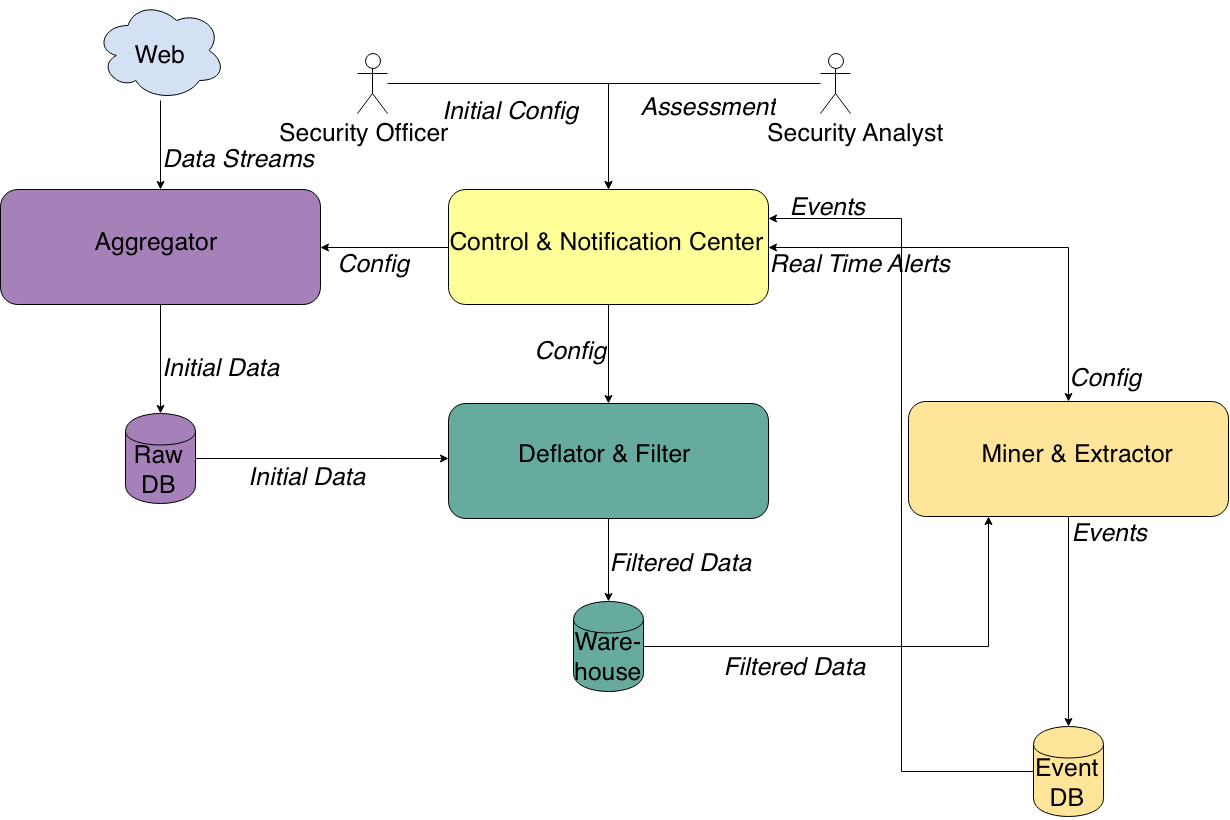
\includegraphics[scale=0.33]{./images/Architecture.png}
    \caption{System Architecture overview}
    \label{fig:arch}
\end{figure}	

\newpage
\subsubsection{Configuration}
The system needs to be as versatile as possible. To that aim each separate part of the system must be able to read a set configuration options that will be inserted into the system through a common control portal. These configuration sets can include (but not be limited to) Data Mining criteria, filtering thresholds, execution intervals for the distinct modules, search keywords, etc. 

\subsubsubsection{Specification}

The configuration set that is most crucial to the operation of the system, is the categorisation of the most common security threats, such as DDoS attacks, malware, exploits and vulnerabilities, etc. This involves the definition of a set of search terms (keywords) associated with each class of threats. Each defined keyword must have an importance level attached to it (weight) denoting the contribution of an occurrence of this word to the score of each document. These keyword lists must follow the format below:\\\\
- Threat Class 1:

keywords: \{[keyword1, weight], [keyword2, weight]...[keywordN, weight]\}\\\\
- Threat Class 2:

keywords: \{[keyword1, weight], [keyword2, weight]...[keywordN, weight]\}
.\\
.\\
.\\
- Threat Class N:

keywords: \{[keyword1, weight], [keyword2, weight]...[keywordN, weight]\}
 
\hfill \break \\
The next step is to define the sources of information. This can be a very cumbersome task that demands expert knowledge and experience, as well as extensive field survey. This study focuses on data originating from public web sources. This can include websites dedicated to one or more security threats as well as social media (Twitter, Facebook, etc.) where general discussions take place. The source list must have a standard format as well:\\\\
- Threat Class 1:

sources: \{[url1, type], [url2, type]...[urlN, type]\}\\\\
- Threat Class 2:

sources: \{[url1, type], [url2, type]...[urlN, type]\}\\
.\\
.\\
.\\
- Threat Class N:

sources: \{[url1, type], [url2, type]...[urlN, type]\}\\\\
Having mentioned that we can distinguish two separate categories of sources which we will name 'Targeted' and 'General'. Targeted sources are websites that provide real time information about security related issues. These sources usually provide their information in a format that is structured to some extent. Their constant monitoring can be used to raise alerts without much further processing.
\hfill \break \\
General sources are much more unpredictable and unstructured. The data collected from such sources have to be further processed in order for the system to distinguish the important from the not important documents as well as to look for previously unknown patterns hidden in the dataset. 
\hfill \break \\
We also need to monitor the names of certain companies or organisations for which the service will be provided. Moreover, we would need to look for several software and hardware vendor name to discover vulnerabilities and known malfunctions for software tools and machinery that are used by companies and organisations. Thus the last thing the operator has to specify is a list of Clients and Vendors. These list must also have weights attached to them, which, however, must be the same for all their members. 
\hfill \break \\
At this point it is useful to mention that we also can monitor certain 'anti-keywords' with negative weights to sort out irrelevant information. For example the word 'attack' might be correlated with the word 'football' or the word 'bug' can be correlated with the word 'insects'. This is a good indication that the subject of the document is probably not security related. 

\paragraph{Keyword Definition}
\hfill \break \\
As it has been mentioned before, it is fundamental to be able to detect different threat types and define the associated search keywords and their weights correctly. In order to be able to select the relevant keywords we can inspect security related news \cite{list-2015-attacks} or discussions related to specific threats. Those keywords that carry most information must be assigned bigger weights. In contrast, commonly appearing words should have a lower weight associated with them since they carry less information.  
\hfill \break \\
For example we can select three of the most common and popular security threats\cite{owasp} and associate a possible list of keywords to them. 
\begin {table}[h!]
\label{tab:title} 
\begin{center} 
\begin{longtable}{|l | l|}
\hline
Type of Attack & Related keywords \\ 
\hline
 Denial-of-Service (DoS) & ddos attack \\ 
 						& take down website \\ 
 						&  server/computer crush  \\
 						& server take down \\
 						& ... \\

\hline
SQL Injection 	& plain text password\\
				& clear text password \\
				& plain text password username \\
				& clear text password username\\
				& dump customers \\
				& dump passwords \\
				& blackmail dump accounts \\
				& leaked passwords \\
				& ... \\
				
\hline
Account hijacking & account hacked \\
				  & account images changed hack \\
				  & take control account \\
				  & account add/remove content \\ 
				  & ... \\	
\hline
... & ...\\		  
\hline
\end{longtable}
\caption {The table contains some example keywords related to possible attacks. When used in combination with a Client or Company Name they might indicate an upcoming or past attack.}
\end{center} 
\end {table}
\newpage
\paragraph{Source Definition}
\hfill \break \\
Discovering real time threats within an accepable margin of error, is a challenging task. One of the reasons is that the Web is essentially an enormous database filled with random information. Within this chaoitic data space, big amounts of security related knowledge can be discovered. Therefore, it is vital to be able to define the reliable sources that can provide valuable information that will allow us to build Security Intelligence. 
\hfill \break \\
The question might arise, which sources can be considered as reliable? In order to answer this question expert knowledge has to be gathered. At this point we were provided with a list of possible sources compiled by the developers of the CTI portal in Deloitte. Among all the possible raw data sources, four were recommended to collect a certain amount of data to be used as a testbed.These are Phishtank, Pastebin, Twitter and Reddit. The impotance level of the above websites can be seen via the fact that critical vulnerabilities were revealed through posted messages\cite{list-2015-attacks}.\\

Since this project is focused on the public Web, other sources such as RSS feeds or IRC channels will not be investigated due to time limitations.   

\subsubsubsection{Implementation}
There has been no implementation effort from our side on this particular system module. However, as it has been mentioned before, there is ongoing effort inside the company towards the development of a CTI portal which will be in essence a configuration provider for the rest of the system. This project proposes the integration of the suggested system with the aforementioned CTI portal that will act as the configuration module. 

%%====DATA AGGREGATION====%%

\subsubsection{Data Aggregation}

After the desired configuration options have been submitted, the  system can start its operation by collecting raw data from the various specified sources. Since we are dealing with more or less unstructured data, some first form of structure must be given during this step.

\subsubsubsection{Specification}

The corresponding module will be composed of several agents, each one responsible for a different source of raw data. Each agent must read its configuration from the appropriate file which will be of a certain format for all the agents. The configuration file will contain information such as the source code directory of the specific agent, associated API keys, the type of each retrieval method (e.g. request based, streaming, etc.), the time intervals that each must be executed etc. Sensitive data such as API keys and Passwords, must be kept in a separate, protected file.
\hfill \break \\
This module will also be responsible for filtering out unrelated information such as profile pictures and uninteresting user details (Twitter, Facebook, etc.) or surrounding html code for sources that have no other means of collection rather than traditional scraping.
\hfill \break \\
As it has been mentioned before some structure can be given at this point to aid further processing. Text based documents, however, must be kept as close to the original content as possible so that if manual inspection is needed the document can be retrieved even if the related Web Resource has been removed.


\subsubsubsection{Implementation}

This module was developed as a collection of separate agents, each aggregating a different web resource. Special care had to be given so that this part is easily extensible. If a developer needs to develop new agents for new sources, they will be presented with a uniform interface that will allow them to include the new agents to the system with minimal effort. 
\hfill \break \\
A tool chaining script was written to allow the agents to be triggered simultaneously and share common configurations. 
\hfill \break \\
The script reads the list of available agents and loads their respective configuration options. It then parses the parameters given by the user regarding which agents need to be run and at what time interval. If the user provides no parameters then the default configuration options are chosen. The user can specify if they need a certain agent not to be executed by passing a -1 parameter. The script reads all the agents selected for execution and loads their source code dynamically on runtime. This last step accounts for extensibility. 
\hfill \break \\
The system must be in a way to determine if the agent opens new connections per request or runs over a persistent connection (e.g. streaming). This must be specified in a common configuration file that lists all the agents. In our particular example this file is formatted in YAML. 

\paragraph{Twitter}
\hfill \break
Twitter exposes both Streaming and RESTful APIs. While the RESTful approach requires separate HTTP connections for each request to the API, Streaming requires keeping a persistent HTTP connection open \cite{twitteroverview}.
\hfill \break \\
For our example we selected the Streaming API approach which provides developers with low latency access to Twitter's global stream of Tweet data \cite{twitteroverview}.
\hfill \break \\
Connecting to the Streaming API requires authentication via an OAuth signature. To generate this signature the user has to register their application and generate four parameters named Consumer key, Consumer secret, Access Token and Access token secret.
\hfill \break \\
One particular endpoint, provided by the Public Stream \cite{twitterpublic}, was used, namely "POST statuses / filter". This endpoint can be reached via the following URL:\url{https://stream.twitter.com/1.1/statuses/filter.json}.
\hfill \break \\
Status filtering allows the user to retrieve tweets that contain certain keywords (up to 400 keywords can be specified), follow specific Twitter users (up to 5000 different users) or retrieve tweets originating from a specific location \cite{twitterfilter}.
\hfill \break \\
In our demonstration we only used the keyword (track) option in order to track specific tweets containing security related words (e.g. attack, hack, vulnerability, etc.)
\hfill \break \\
The data returned from this particular API call are JSON fomated.
\hfill \break \\
The Twitter aggregation agent was developed with the use of Tweepy \cite{tweepy}, an external Python library that provided OAuth authentication and connection to the streaming API.\\ This agent reads its configuration from an external YAML file. This includes Authentication credentials, as well as the specific keywords that we want to track.
\hfill \break \\
The sofware parses the returned JSON object, scrapes all unnecessary information (user profile pictures, background colors, etc.) and stores the rest of the information in the database.  

\newpage
\paragraph{Pastebin}
\hfill \break\\
\textit{Pastebin} websites \cite{fpaste} \cite{pastebin} allow everyone with or without registration to share blocks of text or code snippets. They have attracted many users during past years including cybercriminals such as malware developers\cite{pastebin-magazine}. The enormous flow of information ranges from database dumps, containing e-mails and passwords, to harmful backdoor programs. With a deeper examination of these publicly pasted messages possible future attacks may be discovered.
\hfill \break\\
From all possible \textit{pastebins} (e.g. fpaste.org \cite{fpaste}, paste2.org, pastie.org\cite{pastebin-pastie}, 
paste.ubuntu.org.cn \cite{pastebin-ubuntu} etc.) pastebin.com \cite{pastebin} has been selected to be further inspected.
\hfill \break
\\
Pastebin exposes an API that offers different options for developers. More specifically these include creating new pastes, listing trending pastes or the posts of a particular user. The above functionallities can be used once one obtains a unique Developer API Key. 
\hfill \break
\\
At this moment Pastebin API \cite{pastebin} does not offer any option for listing all new messages posted by unregistered users. The only option available, is to list the posts of a specific registered user. However, any information posted might be of potential interest. 
This makes our work rather challenging but not impossible.  
\hfill \break
\\
One could possibly use the search method provided by \textit{Pastebin.com} for retrieving posts containing a combination of keywords.
This functionality, however, makes use of \textit{Google Custom Search}. Therefore, if one desires to retrieve all posts related to certain specified keywords, they would have to use the Google custom search API. This, however, limits free users to 1000 searches per day. 
\hfill \break
\\
To overcome the above limitations and collect all new pastes that arrive, a web crawler module was implemented. \textit{Scrapy} \cite{scrapy}, an open source framework for building extensible webcrawlers was used, integrated into a Python script. Pastebin's \texttt{Archive} page contains all pastes posted during the last 10 minutes. For that reason, we will crawl and fetch the contents of this page each 10 minutes. Not all data from the page provides interest this is why we will scrape the html and keep only the information that is relevant for further examination. This includes the url, the paste, the posting date and the number of unique views. By inspecting the elements required from the DOM tree, we then can parse these nodes and extract only the raw paste text. Once all this data has been gathered, it will be stored in the database.

\paragraph{Phishtank}
\hfill \break\\
Phishtank is the only 'targeted' source that we examined in this project. It is a website dedicated to tracking Phishing attempts. Any registered user can submit websites that they suspect of Phishing. Other users can log in later and verify if the website is indeed Phishing or not. Phishtank also informs the user if the website is still online or not.
\hfill \break\\
Developing over the Phishtank API is pretty simple and straight forward. Phishtank offers its whole database to be downloaded either in CSV, JSON, XML or serialised PHP format. The database includes all websites that are verified as phishing and are still online, and it is updated every hour. The user is advised to register their applications and obtain an access token in order not to be constricted by download limits.
\hfill \break\\
The aggregator code simply downloads the whole database from the following url \url{http://data.phishtank.com/data/online-valid.json}, parses the json entries and stores in the database all useful information. 
\hfill \break\\\
Since Phishtank is a targeted source, all returned information can be handled directly from the system in order to raise security alerts without much further processing. 
 
\paragraph{Reddit}
\hfill \break
\\
The Reddit community comprises of social media and news sites. It contains over 5000 channels called "subreddits" which belong to different categories. In this project we will collect Reddit \cite{reddit} data originating from the following subreddits:
\begin{itemize}
\item /r/blackhat \cite{r.blackhat}
\item /r/malware \cite{r.malware}
\item /r/netsec \cite{r.netsec}
\item /r/pwned \cite{r.pwned}
\item /r/vrd/ \cite{r.rvd}

\end{itemize}
\hfill \break
\\
Although the Reddit API \cite{reddit} provides a rich list of methods, we have chosen a few of them for the purposes of this project.\\
\hfill \break
In order for a user to list new, top, controversial, etc. messages they would just have to add "/" and the name of the operation they want to perform to the end of the subreddit url in question. The user can provide additional parameters in order to filter, sort, and limit the number of posts retrieved. 
\hfill \break
\\
All ingredients needed for implementing an aggregation agent for Reddit are supplied by the API. The only part we need to add is some filtering capabilities that will allow us to keep the parts of the information that can help with defining the relevance of each document.
\hfill \break
\\
First a connection needs to be opened to the the targeted subreddit, for example /r/blackhat. This is what the following line of code does:

\begin{spverbatim}
response = urllib2.urlopen('http://www.reddit.com/r/blackhat/new
			.json?sort=new&limit=100')
\end{spverbatim}
\hfill \break
\\
The response will be a JSON formatted string. From all the fields in the structure we will only store the title, the number of comments and score. It is important to also store the date of each retrieved message, in order to monitor its voting trends within a specific time period.
\hfill \break
\\
All the collected data are stored in the database. 

\newpage
\subsubsection{Preprocessing and Filtering}
The documents collected from all the public sources must be given a common format suitable for further analysis. Also the system must be able to easily distinguish which documents carry importance for further Security Analysis. 

\subsubsubsection{Specification}
We propose a 'deflation' and scoring model that will help reduce the raw data into a common format as well as help determine the documents that present interest for further analysis. 
\hfill \break\\
The proposed model works in a very targeted and aggressive way, counting the occurrences of each predefined word and deflating the whole document to a list of these keywords. 
\hfill \break\\
Then it multiplies the number of occurrences of each keyword with its associated weight and produces the score for each document. If that score passes a certain predefined threshold the document is marked as interesting and it is moved in its deflated format into the warehousing database. 
\hfill \break\\
The proposed format for the deflated documents is the following:\\

\{document: "DocID", keywords: \lbrack \lbrack keyword1, occurences\rbrack,\lbrack keyword2, occurences\rbrack, ..., \lbrack keywordN, occurences\rbrack \rbrack\,vendors:\lbrack\lbrack vendor1, occurences\rbrack, \lbrack vendor2, occurences\rbrack, ... \lbrack vendorN, occurences\rbrack  \rbrack, clients :\lbrack\lbrack client1, occurences\rbrack, \lbrack client2, occurences\rbrack, ... \lbrack clientN, occurences\rbrack  \rbrack\, score: "score"\}

\hfill \break\\
Certain issues have to be taken into account when following the above approach. First of all we have to make sure that even one occurrence of a client's name will mark the document as interesting. That can be achieved either by associating the client list with a weight higher than the threshold or by performing binary checks for the occurrences of client names (is present or not). 
\hfill \break\\
It is also possible that many occurrences of a certain keyword, even if its importance level is minimal, can mark a certain document as interesting even though it carries no interest. This can be avoided by performing more sophisticated checks by calculating the entropy of each document. This however falls out of the scope of this research.
\hfill \break\\
It also becomes apparent that since this approach creates documents containing only the predefined keywords, other interesting but previously unknown keywords, might be filtered out. Certain ways to mitigate this problem are described in the next sections. 

\subsubsubsection{Implementation}
To test this approach we created a few thousands of fake documents containing random computer terminology, using a free python script called 'Bullshit Generator' \cite{bullgen}. We slightly modified the script to include certain additional keywords as well as to produce exactly 10000 documents and store them in our database. 
\hfill \break\\
We tested the previously defined model to test its efficiency and time consumption. For 10000 documents the code takes less than one second to run, thus we believe that this model can easily be used in any realistic ammount of data. An example output produced by one execution of the software can be seen in Figure~\ref{fig:deflate}

\begin{figure}[t]
\begin{footnotesize}
\begin{spverbatim}

{'count': [['amro', 4], ['apple', 3], ['exploit', 0], ['vulnerability', 0], ['attack', 0], ['ddos', 0], ['deloitte', 0], ['ing', 4], ['bug', 0]], 'doc': ObjectId('54d0bf08aa4ece1e08930ec6'), 'score': 110.0}
{'count': [['amro', 3], ['apple', 2], ['exploit', 2], ['vulnerability', 1], ['attack', 0], ['ddos', 3], ['deloitte', 2], ['ing', 3], ['bug', 0]], 'doc': ObjectId('54d0bf09aa4ece1e08930f3e'), 'score': 109.0}
{'count': [['amro', 2], ['apple', 6], ['exploit', 0], ['vulnerability', 2], ['attack', 1], ['ddos', 1], ['deloitte', 1], ['ing', 1], ['bug', 0]], 'doc': ObjectId('54d0bf09aa4ece1e08930fb4'), 'score': 105.0}
{'count': [['amro', 3], ['apple', 3], ['exploit', 3], ['vulnerability', 0], ['attack', 0], ['ddos', 0], ['deloitte', 1], ['ing', 5], ['bug', 0]], 'doc': ObjectId('54d0bf09aa4ece1e08930ff1'), 'score': 122.4}
{'count': [['amro', 4], ['apple', 2], ['exploit', 2], ['vulnerability', 0], ['attack', 1], ['ddos', 2], ['deloitte', 1], ['ing', 4], ['bug', 0]], 'doc': ObjectId('54d0bf09aa4ece1e08931039'), 'score': 115.8}
.
.
.
\end{spverbatim}
\end{footnotesize}
\captionsetup{font=small}
\caption{Deflation example with a threshold of 100}
\label{fig:deflate}
\end{figure}
\newpage 
\hfill \break
The above results are produced after applying a threshold of 100. This is probably an unrealistic scenario, however.
\subsubsubsection{Alternative Approaches}
Besides the previously mentioned deflation method we have also tested different options. This subsection will outline some alternative methods for cleaning documents by employing NLP techniques as well as the use of the TF-IDF algorithm for determining the relevance and importance of each document.
\newpage
\paragraph{Natural Language Processing}
\hfill \break\\
\parbox{\linewidth}{
Natural Language Processing consists of numerous different tasks such as automatic summarisation, parsing, relationship extraction, topic segmentation and recognition, part of speech recognition, etc.
\hfill \break
\\
Although all of the aforementioned functionalities are important for text processing, part-of-speech tagging in particular can be used in our case to distinguish the meaning of a certain fragment of text. Being able to tell if a certain word is a noun, verb or adjective can help discover the importance of that specific word within a specific topic.  We are mostly interested in distinguishing the nouns since they determine the topic of a sentence.}
\hfill \break
\\
Compared to the suggested deflation method, this technique does not require specifying certain keywords beforehand. This is mainly due to the fact that it allows us to build structured data tables or trees in order to extract the meaningful entities. 
\hfill \break
\\
The aggregation module collects unstructured data, thus in order for us to get the meaning of a certain block of text and determine its relevance, we would have first process it and give it structure. 
\hfill \break
\\
The first step would require removing all stop words such as \textit{the, an, a, about, what, where, etc.} This list can be further expanded to contain any word that one would consider not important, such as numbers, punctuation marks, technical abbreviations (e.g. http), etc.
\hfill \break
\\
Another task called \textit{Stemming} performs suffix removal on verbs, adjectives, etc. 
\hfill \break
\\
We tested how this process works by applying it on posts from \textit{pastebin.com}. However, since lots of pastes contain pieces of source code it is a cumbersome task attempting to recognize different topics, especially after removing the stop words. Previous research papers \cite{second} have shown promising results if the methods described are applied on grammatically correct structured articles. For this reason we tested them on data originating from \textit{Reddit.com}.
\begin{figure}[h]
\begin{footnotesize}
\begin{spverbatim}
----------------------------------------------------
http://www.youtube.com/watch?v=wLtREbONtuI 

----------------------------------------------------
business phone line hacked, calls intercepted. no record or
knowledge of calls in the system. how was it done?
--------------------Analyze-------------------------
Searched word appeared :  1  times
This post has  15  score
And it got  :  10  comments
===================NLTK=============================
	Num Sentences:           3
	Num Words:               23
	Num Unique Words:        21
	Num Hapaxes:             19
	Top 10 Most Frequent Words (excluding stop words):
		system (1)
		business (1)
		calls (2)
		knowledge (1)
		intercepted (1)
		phone (1)
		done (1)
		hacked (1)
		line (1)
		record (1)
\end{spverbatim}
\end{footnotesize}
\captionsetup{font=small}
\caption{NLTK result applied on \textit{Reddit} data}
\label{fig:nltk}
\end{figure}
\hfill \break
\\
\\
The Natural Language Toolkit \cite{nltk} can be integrated into Python code. It provides methods that allow working with \textit{human language data}. We used a few of the functions provided to perform sentence counting, total words counting and most frequent words determination.  The result, seen in Figure~\ref{fig:nltk}, includes the following: the posted URL, the title associated to it, and the output of the nltk process. In this particular example, a keyword search was first performed to find the posts that contain the word \textit{hacked}. For these messages the produced results can be used to determine their importance level, by producing statistical view of the keywords that appear in the text. Using the gathered knowledge and by exploring more NLP capabilities we can determine the importance level of separate posts.
\newpage
\paragraph{TF-IDF}
\hfill \break
\\
TF-IDF \cite{tf-idf} stands for \textit{Term Frequency-Inverse Document Frequency} and it is used to statistically score the importance of a word in a document or across a collection of documents. A word will be considered important if it appears multiple times into a document. TF is calculated by counting how many times the specific word appears, over the total number of words within that document. If that word appears in other documents as well it will be less unique and thus receive a lower score. That score refers to the IDF calculation. 
\hfill \break 
\\
To determine the documents most relevant to specific keywords, it is first required to define certain query terms relevant to known threat categories. The algorithm will take the query into account and will produce a statistical list of the most significant documents as a result. This is an automated method for sorting document importance according to a specified search term. 
\begin{figure}[h!] 
\begin{footnotesize}
\begin{spverbatim}
Overall TF-IDF scores for query 'attack hack'
54c009ecd177b4682d5165c1 0.0801762787248
54c00c7ad177b4685475c1d8 0.113754378362
54c00c82d177b4685475c1e5 0.0875609359758
54c01232d177b4687bd24088 0.123999337904
54c014ddd177b4689699a889 0.0375967860687
54c01d5ad177b468f5807552 0.151241616685
54c0cf17d177b46fa541e070 0.0361664735552
54c0cf24d177b46fa541e084 0.0373855681694
54c0d1a8d177b46ff35304b8 0.0375967860687
54c0d1bfd177b46ff35304dd 0.0375967860687
54c0d9c6d177b470832e5407 0.120993293348
54c0e83bd177b47185269e51 1.98389124491
54c0eae7d177b4719596d5df 0.0924254324189
54c0ee14d177b471b6f3f212 0.0489311112806
54c22910d177b47c8bc1e305 0.0403310977828
54c2613fd177b47f785493eb 0.0891636514564
54c662c3d177b4279d30aecd 0.0610516617813
54c69aefd177b429c8745051 0.193550365357
54c75a8dd177b431883f5d1b 0.495972811226
54c75ff7d177b431d9186d0d 0.0373855681694
54c76b2ed177b432825caf8a 0.0545461568374
54c76e02d177b432b0ca7d0b 0.610428075355
54c7e373d177b43790433dde 0.0386897158963
\end{spverbatim}
\end{footnotesize}
\captionsetup{font=small}
\caption{Overall TF-IDF Result applied on \textit{Pastebin} data, that specifies document ID with the associated score, for the query terms \texttt{attack, hack}}
\label{fig:overall}
\end{figure}
To test how this algorithm actually works we applied it on approximately 5000 real messages gathered from \textit{pastebin.com}. We queried the database to get the total number of documents in the collection:

\begin{spverbatim}
> show collections
system.indexes
pastebin
> db.pastebin.count()
5141
\end{spverbatim}
\hfill \break 
We chose as our main query terms words such as \texttt{attack} and \texttt{hack} to see how the algorithm will behave and which documents are possibly associated with our search. Due to implementation misconfiguration the execution took longer then expected. Considering that our main purpose was to test Data Mining algorithms we did not perform a more profound analysis of the code.

\begin{figure}[h!] 
\begin{footnotesize} 
\begin{spverbatim}
....
TF Doc: 54c0d9c6d177b470832e5407 0.0181818181818 -> attack
TF Doc: 54c00c7ad177b4685475c1d8 0.017094017094 -> attack
TF Doc: 54c01d5ad177b468f5807552 0.0227272727273 -> attack
TF Doc: 54c009ecd177b4682d5165c1 0.0120481927711 -> attack
TF Doc: 54c0d1bfd177b46ff35304dd 0.00564971751412 -> attack
TF Doc: 54c0d1a8d177b46ff35304b8 0.00564971751412 -> attack
IDF:  attack -> 6.65463113416
TF_IDF:  54c662c3d177b4279d30aecd attack -> 0.0610516617813
TF_IDF:  54c014ddd177b4689699a889 attack -> 0.0375967860687
TF_IDF:  54c7e373d177b43790433dde attack -> 0.0386897158963
TF_IDF:  54c00c82d177b4685475c1e5 attack -> 0.0875609359758
TF_IDF:  54c0eae7d177b4719596d5df attack -> 0.0924254324189
TF_IDF:  54c0cf24d177b46fa541e084 attack -> 0.0373855681694
TF_IDF:  54c01232d177b4687bd24088 attack -> 0.123999337904
....
\end{spverbatim}
\captionsetup{font=small}
\caption{A sample from the complete TF-IDF algorithm result. For each function the documentID with associated score and query word is provided}
\end{footnotesize}
\end{figure}
The main reason that contributes to high computational costs was the function that multiplies the TF with the IDF scores and produces the overall score. For 5141 messages the total execution time came to around 15 minutes. If we just calculate the TF and IDF scores the algorithm will run in the following time values: 
\begin{spverbatim}
real	0m0.694s	;	 	user	0m0.508s	;	sys	0m0.023s
\end{spverbatim}
\hfill \break
However costly, this method still provides a good statistical view on the importance of the documents associated to the specified keywords. 
\hfill \break \\
What is actually interesting here is to look at the documents that are included in the \texttt{Overall TF-IDF scores for query "attack hack"} section (Figure~\ref{fig:overall}). The document with the highest score (the ones with a score greater than 1 should not be considered), is the most relevant. In this example it is the document \texttt{54c76e02d177b432b0ca7d0b} with a  score equal to 0.610428075355 (Figure~\ref{fig:android}).
\hfill \break 
\begin{figure}[h!]
\begin{footnotesize}
\begin{spverbatim}
> db.pastebin.find({_id:ObjectId('54c76e02d177b432b0ca7d0b')})
{ "_id" : ObjectId("54c76e02d177b432b0ca7d0b"), "url" :
 "http://pastebin.com/QNxg2fGz", "uniq_visitors" : [ "152" ],
  "paste" : [ "http://besthacksgames.com android cheat engine cheat engine for android cheat engine android android games hack cheat engine 5.5 android game hack android game hacks android cheat engine" ], "time" : [ "Tuesday 27th of January 2015 04:51:41 AM CDT" ] }
\end{spverbatim}
\end{footnotesize}
\captionsetup{font=small}
\caption{MongoDB result when retrieving the document which has \texttt{ID: 54c76e02d177b432b0ca7d0b} with the associated fields \texttt{url, paste, uniq\_visitors and time}, that has a higher score for the word \texttt{hack}}
\label{fig:android}
\end{figure}

\begin{figure}[h!]
\begin{footnotesize}
\begin{spverbatim}

> db.pastebin.find({_id:ObjectId('54c0d9c6d177b470832e5407')})
{ "_id" : ObjectId("54c0d9c6d177b470832e5407"), "url" :
 "http://pastebin.com/dKnHTH1H", "uniq_visitors" : [ "147" ],
  "paste" : 
 	[ "<!DOCTYPE html> <html>    <head>      <title>Scripting Attack 						Demo</title>        <link />        <script>       
   	// find out the location url      
   	 name=decodeURIComponent(window.location.search.substring(1)); 
   	 console.log(name); name=fred is the sort of thing we expect to append... 
   	 //
    	 script alert  You are under
    	  attack /script     
    	  or this...  script src=siteB/evil.js /script         
     	 // a trivial fixer        
     	 name = name.replace(/</g, \"&lt;\").replace(/>/g, \"&gt;\");                    document.write('Hello ' + name);      
        </script>        <meta />   </head> <body></body></html>" ], "time" : [ "Thursday 22nd of January 2015 05:02:13 AM CDT" ] }
\end{spverbatim}
\end{footnotesize}
\captionsetup{font=small}
\caption{MongoDB result when retrieving the document which has \texttt{ID: 54c0d9c6d177b470832e5407} with the associated fields \texttt{url, paste, uniq\_visitors and time},that has a lower score for the work \texttt{attack}}
\label{fig:script}
\end{figure}
\hfill \break 
The word \texttt{hack} appears four times in this text(Figure 2.5), and is considered to have a higher value.
If we analyse another document(Figure 2.6) for example the one with ID :  54c0d9c6d177b470832e5407, that has an associated score of  0.120993293348, it presents a lower score we see that the word \texttt{attack} appears less then four. However not only the frequency of the word \texttt{attack} in this text is taken in consideration but also its frequency across all documents.\\
\hfill \break 
\newpage
\subsubsection{Analytics and Alerting}

After the data has been collected and preprocessed into a common format it can be analysed in order for Security Intelligence to be extracted.  This will be achieved by employing various Data Mining tasks and using their output to create Security Incident alerts. 

\subsubsubsection{Specification}
Data Mining is the analysis step of the Knowledge Discovery in Databases (KDD) \cite{datamining}. Its aim is to extract previously unnoticed patterns and behaviours within the data set. Data mining involves six common classes of tasks \cite{datamining}. These tasks are described below and the manner they fit our use case is described briefly. The tasks that have been tested are described in further detail. 

\paragraph{Data mining tasks}
\begin{itemize}
\item 
\textbf{Classification}: Refers to the task of generalising known structures and applying them to new
data. For example, an e-mail program might attempt to classify an e-mail as "legitimate" or as
“spam”. Since this involves training of the algorithm before use, it might not be ideal for use in
threat discovery. However, it can be very useful for providing feedback to the system and fine
tuning it to be able to classify the documents for each threat category, acting together with the
configuration step
\item 
\textbf{Anomaly detection} (Outlier/change/deviation detection): This task refers to identification of
unusual data records that might imply unusual behaviour in the dataset. For example, in our
use case, a first indication that something might be possibly wrong would be an exceptional
mention of a company name within a certain period of time. The problem here is to determine
what can be defined as exceptional. This of course is not possible without the use of old data
so a certain threshold can be determined. Until sufficient amount of data has been gathered we
can naively implement this by setting the thresholds manually. This operation is particularly
popular in intrusion detection systems.
\item 
\textbf{Association rule learning} (Dependency modelling): This task refers to the search for
relationships between variables. One example of this is the infamous beer and diapers story.
This test requires no training set and can be performed on any structured set of data. In our
use case this can help us determine trends between the occurrences of keywords, such as the
name of a company together with the name of a name of an attack. The output of this test also
contains metrics about the support (percentage of the documents supporting the association) as well as
confidence (ratio of the support percentage of either part of each rule).
\item 
\textbf{Clustering}: Refers to the task of discovering groups and structures in the data that present
some sort of similarity, without using known structures in the data. In our case this can help us
determine new categories of documents that have not been predefined (remember the threat
categorisation we mentioned in the beginning).
\item
\textbf{Regression}: This task attempts to find a function which models the data with the least error.
This might not be directly applicable to our specific example but based on the experience
gathered after a certain period of time that the system will be operated, we can attempt to
design an analytic model using regression analysis techniques.
\item
\textbf{Summarisation}: This task aims to provide a more compact representation of the data set, including visualisation and report generation. In our case this applies to the creation of the alerts to be presented to the Security Analysts. The alerting will consist of a common format that will apply to automatically generated events that will be propagated to the appropriate parties. One proposed format could be the following:
%\{alert\_id: 00001, subject: "Something is rotten in the state of Denmark", importance: Red, backing_documents:\[1,3,4,6\]\}
This presents the analyst with an event informing them about a security incident with a certain importance level. The way of determining the level of importance falls out of the scope of thisn document. Notice also the list of supporting documents resulting from different sources. At this point the analyst can go and inspect each one of this documents manually, assess the risk themselves and take the appropriate measures such as further informing the involved parties, or ignoring the alert.
\end{itemize}
\subsubsubsection{Implementation}
\paragraph{Association Rule Learning}
\hfill \break 
\\
Association Rule Learning is usually performed on databases that contain sales transactions (e.g. \{milk, butter, bread, jam\}) and for that reason it is sometimes referred to as Market Basket Analysis \cite{assoc1}. However, since we have documents deflated to contain only certain keywords, this method is very suitable to help us distinguish frequent item sets. 
\hfill \break 
\\
The most commonly used algorithm for performing this operation is called Apriori \cite{apriori1}. It  employs a "bottom up" approach, during which frequent subsets are extended one item at a time, a step known as \textit{candidate generation}. All groups of candidates are tested against the data. The algorithm terminates when no further successful extensions can be found. The algorithm produces two part rules that have the format $X \rightarrow Y$. This denotes that when subset $X$ occurs, subset $Y$ is likely to occur as well.  \hfill \break 
\\
We produced an example implementation of the algorithm by using the \texttt{associate}\cite{orange-assoc} package from the \texttt{Orange}\cite{orange} analytics and visualisation framework. The code was tested on actual documents originating from \texttt{Twitter}, deflated against certain keywords.  \hfill \break 
\\
For each association rule produced (Figure~\ref{fig:assoc}), three quantitative statistical measures that denote the importance of the rule. This measures are called \texttt{Support}, \texttt{Confidence} and \texttt{Lift}. Support refers to to the fraction of the documents that contain both $X$ and $Y$ parts of the rule, while Confidence measures how often each item in Y appears in documents that contain X. Lift is an expectance measure denoting the correlation between each part of the rule. A Lift value greater than 1, for example, shows that the two parts of the rule appear together more often than expected, i.e it is more possible to find these two sets together rather than alone. 
\hfill \break 
\\
\begin{figure}[h!]
\begin{footnotesize}
\begin{spverbatim}

 supp    conf    lift,  rule
0.014   0.276   9.196   "exploit" -> "vulnerability"
0.014   0.465   9.196   "vulnerability" -> "exploit"
0.032   0.640   2.165   "exploit" -> "attack"
0.032   0.109   2.165   "attack" -> "exploit"
0.014   0.154   1.072   "charlie" -> "paris"
0.014   0.096   1.072   "paris" -> "charlie"
0.012   0.133   0.960   "charlie" -> "paris" "attack"
0.012   0.865   2.928   "charlie" "paris" -> "attack"
0.012   0.165   1.148   "charlie" "attack" -> "paris"
0.012   0.083   1.148   "paris" -> "charlie" "attack"
0.012   0.086   0.960   "paris" "attack" -> "charlie"
0.012   0.040   2.928   "attack" -> "charlie" "paris"
0.072   0.808   2.735   "charlie" -> "attack"
0.072   0.245   2.735   "attack" -> "charlie"
0.079   0.517   1.565   "password" -> "account"
0.079   0.240   1.565   "account" -> "password"
0.013   0.082   0.340   "password" -> "hacked"
0.013   0.052   0.340   "hacked" -> "password"
0.122   0.758   5.199   "nude" -> "jennifer"
0.122   0.836   5.199   "jennifer" -> "nude"
0.011   0.071   2.197   "nude" -> "jennifer" "leaked"
0.011   0.093   0.701   "nude" "jennifer" -> "leaked"
0.011   0.230   1.580   "nude" "leaked" -> "jennifer"
0.011   0.078   1.580   "jennifer" -> "nude" "leaked"
0.011   0.353   2.197   "jennifer" "leaked" -> "nude"
0.011   0.085   0.701   "leaked" -> "nude" "jennifer"
0.015   0.211   1.584   "sony" -> "leaked"
0.032   0.108   1.479   "attack" -> "sony"
0.032   0.437   1.479   "sony" -> "attack"
0.014   0.185   0.560   "sony" -> "account"
0.014   0.041   0.560   "account" -> "sony"
0.011   0.150   0.623   "sony" -> "hacked"
0.011   0.046   0.623   "hacked" -> "sony"
0.190   0.575   2.392   "account" -> "hacked"
0.190   0.790   2.392   "hacked" -> "account"
\end{spverbatim}
\end{footnotesize}
\captionsetup{font=small}
\caption{Example output of the Association Rule implementation. The first 3 columns show the \texttt{Support}, \texttt{Confidence} and \texttt{Lift} for each produced rule.}
\label{fig:assoc}
\end{figure}
\newpage
\paragraph{Clustering}
\hfill \break 
\\
For our specific use case Clustering is important for automating the process of finding new types of Security Threats that arise during a specific period of time. 
\hfill \break 
\\
The method described below, groups documents that refer to a specific topic into clusters and provides a list of the most frequently occurring terms within each cluster.
\hfill \break 
\\
For clustering a number of collected documents within the database in K categories we could use the K-means\cite{k-means} algorithm, also known as Lloyd's algorithm. This algorithm \cite{k-means-example} attempts to find K non-overlapping clusters. It takes the desired number of clusters, K, and selects K initial centroids in a  random manner. Thus the information will be divided into K clusters. It assigns each observation point(word) to its closest centroid, where each collection of points(words) forms a cluster. Within the cluster a new centroid selected by calculating the Euclidean distance between the gathered words. This process runs iteratively and stops when the clusters do not change any more.
\hfill \break 
\\ 
There is no guarantee that the result produced will be optimal. The outcome might differ each time, depending on how the initial centroids have been chosen. An important factor that we need to mention at this point is the selection of number K, as an incorrect choice might lead to non-optimal results. There are several procedures\cite{procedures-for-kmeans} for calculating the favourable number of clusters but this is out of scope of this project. For this example we will chose the number of clusters that will make sense compared to the amount of data gathered.
\hfill \break 
\\
In order to implement the proposed algorithm the free and open source scikit-learn \cite{sklearn} toolkit was used. It provides a library collection called SKlearn which can be used in Python scripts. Following an example that attempts to categorize 20 news groups \cite{k-means-20news}, provided as a tutorial at the sklearn website, and adapting it to use our collected data we tried to find out which are the documents related to each other in each cluster. We applied the algorithm on over 600000 messages from Twitter and the expected to have them categorised in 20 groups. From all the clusters obtained, three of them showed considerable interest as they present real world events that took place recently (Figure~\ref{fig:clusters}). 

\begin{figure}[h!]
\begin{footnotesize}
\begin{spverbatim}
Cluster 13:  paris  charlie  hebdo  attack  http  mayor  nypd  
rt  victims  french  honor  visited  nyc  france  terror  muslim 
 bolsters  security  jewish  cover
Cluster 15:  photos  leaked  upton  kate  jennifer  lawrence 
 nude  victoria  justice  megan  fox  http  seen  rt  hoeuu2dubr  
itweetlikegirls  hilarious  kardashian  kim  aigbtbpmvv
Cluster 18: attack http rt titan panic bus hotel tel aviv killed 
terror amp deadly anxiety people terrorist tripoli video use
\end{spverbatim}
\end{footnotesize}
\captionsetup{font=small}
\caption{A sample from the complete K-means Clusters Result produced from  600000 messages originated from \textit{Twitter.com} }
\label{fig:clusters}
\end{figure}
\hfill \break
By inspecting the clusters that the algorithm produced we can say with some certainty that the algorithm behaved well considering that it is an unsupervised method.
We can clearly see that top frequent terms for Cluster 13, highlight the recent attack in Paris\cite{hebdo}. Also Cluster 15 is totally unrelated to the previous topic, and instead refers to the incident of the leaked celebrity photos\cite{fappening}. The same with Cluster 18 that discusses a terrorist attack in Israel\cite{tel-aviv}.  

\paragraph{Classification}
\hfill \break
\\
We used classification task to map specific data into categories such as certain threats or attacks. Because we have to classify the information given into multiple categories, we selected multi-label classification\cite{classiciation-multilabel} to implement this method. In this case we have to train each class corresponding to a label. To showcase how it works and that is a feasible attempt, we constructed a training set that contains a list of sentences as it can be seen in \textit{Figure 2.9}. In each sentence there might or might not be an \textit{attack} explicitly specified, as it belongs to a certain class that will be added to the training list.  The targeted categories are the following : \texttt{ddos,xss,spoof} with the associated number list \texttt{\{0,1,2\}} . The algorithm attempts to recognize patterns for the new incoming sentences by checking the list to which we associates corresponding numbers.    

\begin{figure}[h!]
\begin{footnotesize}
\begin{spverbatim}
X_train = np.array(["On the following site there is evidence of ddos attack ",
                    "a lot of attacks have been ddos encountered",
                    "some attacks are not only ddos or xss",
                    "ddos will make your computer impossible to use",
                    "e-mail addresses for spoofing",
                    "there has been noticed some spoofing action",
                    "someone's email got spoofed",
                    "spoofing is for attackers fun",
                    "nothing can compare with ddos attack and spoofing same time",
                    "some ddos and spoofing has been monitored",
                    "I just want to type something spoofing more about ddos"])

y_train = [[0],[0],[0,1],[0],[2],[2],[2],[2],[0,2],[0,2],[2,0]]
target_names = ['ddos', 'xss','spoof']

\end{spverbatim}
\end{footnotesize}
\captionsetup{font=small}
\caption{A simple example of the built training set with the associated trained list and targeted categories }
\label{fig:trainset}
\end{figure}
\begin{figure}[h!]
\begin{footnotesize}
\begin{spverbatim}
Spoofed addresses found on this site => spoof
ddos lala somewhere in the sky => ddos
hello frm my spoofed mail and here boom ddos attack => ddos, spoof
\end{spverbatim}
\end{footnotesize}
\captionsetup{font=small}
\caption{The result matches to which class the specified label belongs}
\label{fig:trainset-result}
\end{figure}

\newpage
\subsubsection{Feedback and Assessment}
During the last step of the operation the system will have to be able to produce reconfiguration sets in order to adjust its behaviour and produce more accurate results in the future.
\hfill \break\\
At this point a Security Analyst will have to be presented with a way of assessing each alert and  determining the real importance level of each presented event.
\hfill \break\\
Their assessment will be recorded in the events database along with the initial alert record so that the divergence between the estimated and the actual threat level can be calculated. This result will be propagated to the various modules of the system which can afterwards re-adjust their configurable parts to achieve better accuracy.
\hfill \break\\
Unfortunately the exact way of how this is going to be realised, also falls out of the scope of this project due to time limitations. However, we are in a position to suggest that certain Data Mining techniques discussed in the previous sections (e.g. Clustering, Classification, Regression) can be employed during this phase as well. Once large enough training sets have been built these techniques can provide valuable guidelines to the system. 

\newpage
\section{Conclusions}

We have designed and proposed the architecture of a system capable of generate Security Intelligence. We have also specified the distinct modules that compose this system and implemented the most important of them with the aim of building a Proof of Concept and an initial test of the System Architecture. 
\hfill \break\\
We proposed a uniform way of providing initial configuration options for the system. We specified the format that the search terms will be inserted to the system and how their importance levels can be determined. 
\hfill \break\\
We developed aggregation agents for four different Web sources and collected 2GB of data which we used as a test dataset for the next parts of the system. 
\hfill \break\\
We tested different methods for preprocessing and filtering the collected documents. Due to the fact that mature methods such as Natural Language Processing techniques or TF-IDF needed to be investigated more deeply in order to fit our purpose, we instead proposed a different document deflation and scoring method. After putting this method to the test we can conclude that it is fast and efficient enough to be included at the preprocessing phase. 
\hfill \break\\
For the analysis of the collected data we tested several Data Mining tasks, namely Association Rule Learning, Clustering and Classification. The use of the remaining Data Mining techniques in our proposed system was briefly mentioned. The results produced by the tested algorithms were deemed as promising. 
\hfill \break\\
Apparently this system has to be tested thoroughly with real world data and within a significant amount of time so its accuracy and efficiency can be measured. Also its installation and operating costs have to be estimated. 
\hfill \break\\
There is a lot of effort to be invested towards the correct implementation of this system. Several extensions and corrections can be proposed after careful inspection the system operation. 


\newpage
\section{Future Work} 

At this moment we have implemented a modular and pipelined system by using open source tools. As a future extension, one target would be to have a full system implementation. This system can be further integrated with already developed CTI (Cyber Threat Intelligence) portal. Due to the lack of time, we have build a simple training set in the classification module, just to showcase that it is a feasible attempt to categorize a new given set of items based on the previous trained set. A normal step would be to build numerous training sets from the real world data, gathered from social websites, and test them on the new incoming data. This step requires time as new attacks might happen in a week, month or year. Therefore at least one year would be necessary to have a stable, favourable trained set. Classification method can also be used for exploring sentiment analyses for the collected messages. To build a set that will distinguish false positives, at first this can be done manually by a Security Analyst which could split a real attack from just a random message. Moreover, natural language processing capabilities can be explored to filter messages from all the unnecessary data and retrieve only the interesting data that can be further structured for a more detailed analysation. Clustering method that we proposed for finding new categories of attacks that might have been omitted, uses a random K number defined by user. For optimised results, a good solution would be to check the proposed methods for finding the optimal number of clusters in a given dataset. An expected outcome for the assessment module would be the ability to rise real time alerts in the moment a threat or attack to certain company or client is found.



\newpage
\begin{appendices}
\section{Code}
\section{Results}

\end{appendices}

\subsection{Acronyms}


% just trying
%\newglossaryentry{utc}{name=UTC, description={Coordinated Universal Time}}
%\newglossaryentry{adt}{name=ADT, description={Atlantic Daylight Time}}
%\newglossaryentry{est}{name=EST, description={Eastern Standard Time}}
 
% Use the terms
%\gls{utc} is 3 hours behind \gls{adt} and 10 hours ahead of \gls{est}.
 
%Print the glossary
\printglossaries
\newpage

\begin{thebibliography}{99}
\bibitem{cyber}
US cybercrime: Rising risks, reduced readiness, PWC, Available at: \url{http://www.pwc.com/en_US/us/increasing-it-effectiveness/publications/assets/2014-us-state-of-cybercrime.pdf}
\bibitem{sony}
	 D. Sanger, N. Perlroth.  U.S. Said to Find North Korea Ordered Cyberattack on Sony. [online] Nytimes.com. \\Available at: \url{http://www.nytimes.com/2014/12/18/world/asia/us-links-north-korea-to-sony-hacking.html?_r=0}
\bibitem{socialweb}
  Russell, MA (2014). Mining the Social Web, O'Reily Media, USA
\bibitem{minds}
    V. Chandola et al. Data Mining for Cyber Security, Department of Computer Science, University of Minnesota, Springer, 2006
\bibitem{police}
   RCP van der Veer, H.T. Roo,  A. van der Zanden, Data mining for intelligence led policing, Sentient, Amsterdam Police Force, Amsterdam, The Netherlands, 2009
\bibitem{nltk}
Nltk.org, (2015). Natural Language Toolkit - NLTK 3.0 documentation. [online] Available at: \url{http://www.nltk.org/}

\bibitem{fpaste}
Fedora Project Pastebin Fpaste.org, (2015). New paste • Fedora Project Pastebin. [online] Available at:  
\url{http://fpaste.org }
\bibitem{pastebin}
Pastebin, (2015). Pastebin.com - \#1 paste tool since 2002!. [online] Available at:     \url{http://pastebin.com/}

\bibitem{pastebin-magazine}
Security Intelligence, (2015). Pastebin a Convenient Way for Cybercriminals to Remotely Host Malware. [online] Available at: \url{http://securityintelligence.com/news/pastebin-convenient-way-cybercriminals-remotely-host-malware/#.VMS25DX8vCI }
\bibitem{pastebin-pastie}
Pastie.org, (2015). New - Pastie. [online] Available at: \url{http://pastie.org} 
\bibitem{pastebin-ubuntu}
 Paste.ubuntu.org.cn, (2015). [online] Available at: \url{http://paste.ubuntu.org.cn/}
\bibitem{scrapy}
Scrapy.org, (2015). Scrapy | A Fast and Powerful Scraping and Web Crawling Framework. [online] Available at: \url{http://scrapy.org/} 
\bibitem{reddit}
Reddit.com, (2015). reddit: the front page of the internet. [online] Available at: \url{http://www.reddit.com/} 
\bibitem{r.blackhat}
Reddit, (2009). blackhat library: Documenting blackhat hacking techniques • /r/blackhat. [online] Available at: \url{https://www.reddit.com/r/blackhat}
\bibitem{r.malware}
Reddit, (2009). Malware Analysis \& Reports • /r/Malware. [online] Available at:   \url{http://www.reddit.com/r/malware}
\bibitem{r.netsec}
reddit, (2007). /r/netsec - Information Security News \& Discussion. [online] Available at: \url{https://www.reddit.com/r/netsec/} 
\bibitem{r.pwned}
Reddit, (2008). pwned • /r/pwned. [online] Available at: http://www.reddit.com/r/pwned 
\bibitem{r.rvd}
Reddit, (2012). Vulnerability Research and Development • /r/vrd. [online] Available at: \url{http://www.reddit.com/r/vrd/}
\bibitem{oracle-list}
Oracle.com, (2015). Oracle Data Mining Techniques and Algorithms. [online] Available at: \url{http://www.oracle.com/technetwork/database/enterprise-edition/odm-techniques-algorithms-097163.html}
\bibitem{tf-idf}
Tfidf.com, (2015). Tf-idf : A Single-Page Tutorial - Information Retrieval and Text Mining. [online] Available at: \url{http://www.tfidf.com/} 
\bibitem{data-kdd}
Han, Jiawei; Kamber, Micheline (2001). Data mining: concepts and techniques. Morgan Kaufmann. p. 5. ISBN 9781558604896. "Thus, data mining should have been more appropriately named "knowledge mining from data," which is unfortunately somewhat long"
\bibitem{owasp}
Owasp.org, (2015). Category:OWASP Top Ten Project - OWASP. [online] Available at: \url{https://www.owasp.org/index.php/Top10#OWASP_Top_10_for_2013} 
\bibitem{list-2015-attacks}
Passeri, P., Passeri, P. and Passeri, P. (2015). Cyber Attacks Timeline | Hackmageddon.com. [online] Hackmageddon.com. Available at: http://hackmageddon.com/category/security/cyber-attacks-timeline/ 
\bibitem{sklearn}
Scikit-learn.org, (2015). scikit-learn: machine learning in Python — scikit-learn 0.15.2 documentation. [online] Available at: \url{http://scikit-learn.org/stable/index.html}
\bibitem{orange}
Bioinformatics Laboratory, U. (2015). Orange Data Mining. [online] Orange.biolab.si. Available at: \url{http://orange.biolab.si/} 
\bibitem{k-means} Junjie Wu , Advances in K-means Clustering: A Data Mining Thinking
\bibitem{k-means-example}
Gonçalves, H. (2015). K-means clustering - algorithm and examples. [online] Onmyphd.com. Available at: \url{http://www.onmyphd.com/?p=k-means.clustering}
\bibitem{procedures-for-kmeans}    Glenn W. Milligan, Martha C. Cooper , An examination of procedures for determining the number of clusters in a data set
\bibitem{k-means-20news}
Scikit-learn.org, (2015). Clustering text documents using k-means — scikit-learn 0.15.2 documentation. [online] Available at: \url{http://scikit-learn.org/stable/auto_examples/document_clustering.html} 

\bibitem{classiciation-multilabel}
Scikit-learn.org,. '1.12. Multiclass And Multilabel Algorithms — Scikit-Learn 0.16.Dev Documentation'. N.p., 2015. Web. 
 
\end{thebibliography}
\end{document}
